\chapter{Interface et Implémentation - Listes, piles, files}
Ce cours présente de nouvelles façons d'organiser et de traiter les données, que l'on appelle des structures de données. On rencontrera, notamment, des structures linéaires comme la liste, la pile et la file, mais également des structures relationnelles telles que les arbres ou les graphes (à voir dans les chapitres suivant). Dans ce chapitre, nous allons commencer par distinguer la structure de données de son implémentation en illustrant les concepts avec le jeu ricochet robot.\\

\begin{tcolorbox}[enhanced,
    colback=green!25!black!10!white,colframe=green!75!black,title=Structure de données,
    drop fuzzy shadow,watermark color=white]
    Une structure de données est un format pour organiser les données dans le but de les traiter, de les extraire et de les stocker. 
  \end{tcolorbox}


Le choix de la structure de données est important dès qu'on souhaite stocker et manipuler efficacement des données. Le choix se fait en fonction du \textbf{besoin}. Il est donc important de spécifier son besoin pour choisir la structure de données la plus adéquate.\\


\includegraphics[scale=0.03]{Thème 1 – Structures de données/Chapitre 1 - Interface et implémentation/BLOB/mindblow.png}{\fontfamily{cmss}\selectfont
Pourquoi existe-t-il plusieurs structures de données ?\\
}
Le choix de la bonne structure de données permet de gagner beaucoup de temps de calcul. Ainsi, certain programmes ne pourraient pas exister si on utilisait la mauvaise structure de données. En effet, la résolution deviendrait trop longue.\\



Commençons par les structures de données suivantes :
\begin{itemize}
    \item Les listes
    \item Les files FIFO
    \item Les piles LIFO
\end{itemize}

\begin{tcolorbox}[enhanced,
    colback=green!25!black!10!white,colframe=green!75!black,title=Structuress linéaires,
    drop fuzzy shadow,watermark color=white]
Ces trois structures de données sont dites \textbf{linéaires} : les données sont organisées dans un ordre dans lequel les éléments sont liés les uns après les autres.
\end{tcolorbox}

%On différencie l'interface qui est un objet algorithmique spécifiant des méthodes (appelées primitives) pouvant être appliquées sur une structure de données de l'implémentation d'une structure de données dans un langage permettant sa mise en œuvre pratique.


On différencie l'interface de l'implémentation. L'interface va spécifier théoriquement la structure de données en proposant des fonctions qu'on peut appliquer sur la structure tandis que l'implémentation et l'utilisation de ces structures avec un langage de programmation. Voici les définitions formelles :

\begin{tcolorbox}[enhanced,
    colback=green!25!black!10!white,colframe=green!75!black,title=L'interface,
    drop fuzzy shadow,watermark color=white]
    L'interface qui est un objet algorithmique spécifiant des méthodes (appelées primitives) pouvant être appliquées sur une structure de données.
\end{tcolorbox}

\begin{tcolorbox}[enhanced,
    colback=green!25!black!10!white,colframe=green!75!black,title=L'implémentation,
    drop fuzzy shadow,watermark color=white]
    L'implémentation d'une structure de données dans un langage permettant sa mise en œuvre pratique
\end{tcolorbox}

\newpage
\section{Les listes}

Les listes regroupent des données de manière à pouvoir y accéder librement (contrairement aux files et aux piles, dont l'accès se fait respectivement en mode FIFO et LIFO). Comme vu l'année dernière, un tableau peut être représenté par une liste.\\

\begin{minipage}{0.45\linewidth}
    Par exemple, sur l'image ci-contre, à l'index 4, on lit la valeur 31. 
\end{minipage}\begin{minipage}{0.49\linewidth}
    \begin{center}
        \includegraphics*[width=\linewidth]{Thème 1 – Structures de données/Chapitre 1 - Interface et implémentation/BLOB/Tableau_une_dimension.png}
    \end{center}
\end{minipage}


\includegraphics[scale=0.03]{Thème 1 – Structures de données/Chapitre 1 - Interface et implémentation/BLOB/mindblow}{\fontfamily{cmss}\selectfont
Comment les manipuler ?\\
}

On peut manipuler des listes grâce à des fonctions. En voici les \textbf{primitives} :\\

\noindent\begin{tabular}{l | l }
    \textbf{Insérer} & ajoute un élément dans la liste. \textit{Add} en anglais\\
    \textbf{Retirer} & retire un élément de la liste.   \textit{Remove} en anglais \\
    \textbf{La liste est-elle vide ?} & renvoie "vrai" si la liste est vide, "faux" sinon.   \textit{IsNull} en anglais\\
    \textbf{Nombre d'éléments dans la liste} & renvoie le nombre d'éléments dans la liste. \textit{Length} en anglais\\[0.5cm]
\end{tabular}

C'est ce qu'on appelle \textbf{l'interface}.\\


\includegraphics[scale=0.03]{Thème 1 – Structures de données/Chapitre 1 - Interface et implémentation/BLOB/mindblow}{\fontfamily{cmss}\selectfont
Comment les manipuler avec python ?\\
}
\begin{lstlisting}[language=Python]
    # Creer une liste vide 
    l = []

    # Creer une liste non vide
    l = ["gauche", 3, 2.3, 7, "droite"]

    # Taille de la liste
    print(len(l)) # affiche la taille de la liste

    # Acceder a un element par son indice
    print(l[4]) # affiche "droite"

    # Cas particulier
    # Premier element
    print(l[0]) # affiche "gauche"
    # Dernier element 
    print(l[-1]) # affiche "droite"
    print(l[len(l)-1]) # affiche "droite"

    # Ajouter un element
    l.append("haut")
    print(l) # affiche ["gauche", 3, 2.3, 7, "droite", "haut"]

    # Supprimer un element
    del(l[3])
    print(l) # affiche ["gauche", 3, 2.3, "droite", "haut"]
\end{lstlisting}

C'est ce qu'on appelle \textbf{l'implémentation}.\\

\textit{Remarque :} on peut accéder par indice avec des indices positifs en partant du début de la liste ou avec des indices négatifs en partant de la fin de la liste.

    \begin{tabular}{l c c c c c c c}
        liste & : &["A", & "B", & "C", & "D", & "E", &"F"]\\
        indice positif & : & 0 & 1 & 2 & 3 & 4 & 5\\
        indice négatif & : & -6 & -5 & -4 & -3 & -2 & -1\\
        \\
    \end{tabular}

\newpage
\textbf{Exemple avec le jeu ricochet robot}
\begin{center}
    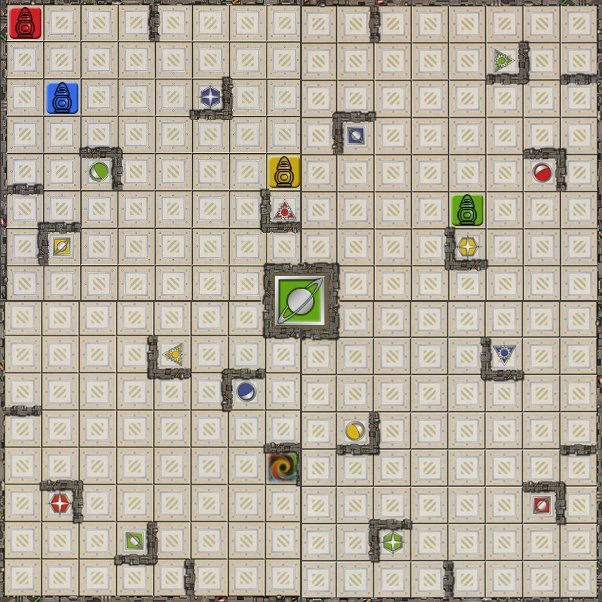
\includegraphics[width=0.7\linewidth]{Thème 1 – Structures de données/Chapitre 1 - Interface et implémentation/BLOB/ricochet-robots-plateau}
\end{center}
Ceci est une grille où peuvent se déplacer les robots. Pour les déplacer on utilise les fonctions "deplacer\_B()", "deplacer\_R()", "deplacer\_J()", "deplacer\_V()", respectivement pour les robots bleu, rouge, jaune et vert.
Ces fonctions prennent en paramètre "haut", "bas", "gauche" ou "droite". Quand on appelle deplacer\_B(), le robot bleu se déplace d'une case dans la direction donnée en paramètre.\\


\underline{Exercice 1:}
\begin{lstlisting}[language=Python]
    D = ["haut", "bas", "gauche", "droite"]

    deplacer_B(D[1])
    deplacer_B(D[1])
    deplacer_B(D[3])
\end{lstlisting}
Sur quel repère se trouve le robot bleu?\\

\underline{Exercice 2:}
\begin{lstlisting}[language=Python]
    D = ["haut", "bas", "gauche", "droite"]

    deplacer_J(D[len(D)-2])
    deplacer_J(D[len(D)-2])
    deplacer_J(D[len(D)-2])
    deplacer_J(D[0])
    deplacer_J(D[0])
    deplacer_J(D[len(D)-1])
\end{lstlisting}
Sur quel repère se trouve le robot jaune?

\newpage
\underline{Exercice 3:}
\begin{lstlisting}[language=Python]
    D = ["haut", "bas", "gauche", "droite"]

    deplacer_V(D[-1])
    deplacer_V(D[1])
    deplacer_V(D[-3])
    deplacer_V(D[len(D)-3])
    deplacer_V(D[4-3])
\end{lstlisting}
Sur quel repère se trouve le robot vert ?\\

\underline{Exercice 4:}
\begin{lstlisting}[language=Python]
    D = ["haut", "bas", "gauche", "droite"]
    a = 2
    b = 3
    deplacer_V(D[a])
    deplacer_V(D[1])
    a = 1
    deplacer_V(D[a])
    deplacer_V("droite")
    deplacer_V(D[b])
    deplacer_V(D[0])
    deplacer_V(D[b-a])
\end{lstlisting}
Sur quel repère se trouve le robot vert?\\

\underline{Exercice 5:}
\begin{lstlisting}[language=Python]
    D = []
    if D :
        print("D est vide !")

    D.append("bas")
    D.append("droite")
    deplacer_R(D[0])
    D[0] = "droite"
    deplacer_R(D[0])
    D.extend("haut","bas","gauche")
    deplacer_R(D[3])
    deplacer_R(D[-2])
    del(D[1])
    if D :
        print("D est vide !")
    else :
        deplacer_R(D[len(D)-2])
        deplacer_R(D[0])
\end{lstlisting}
Sur quel repère se trouve le robot rouge ?\\

\underline{Exercice 6:}
\begin{lstlisting}[language=Python]
    D = ["haut", "bas", "gauche", "droite"]

    deplacer_V(D[2])
    for i in range(1,10) :
        deplacer_V(D[1])
    deplacer_V(D[-2])
\end{lstlisting}
Sur quel repère se trouve le robot vert ?\\

À votre tour de faire jouer les autres. Mettez-vous par groupe de 3 et faites une liste d'instructions pour déplacer un robot. Les autres groupes devront réussir à trouver sur quel repère le robot se trouvent à la fin de votre programme.
% \begin{center}
%     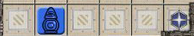
\includegraphics[width=0.5\linewidth]{jeu_ligne}
% \end{center}


\newpage
\section{Les files FIFO et les piles LIFO}

Les files sont adaptées pour stocker des élèments suivant une séquentialité. Les files FIFO suivent la politique "premier entré, premier sorti" (\textit{first in, first out} en anglais). Les premiers éléments ajoutés à la file seront les premiers à en être retirés; tandis que les LIFO suivent la règle "premier entré, premier sorti"(\textit{last in, last out} en anglais).\\


\includegraphics[scale=0.03]{Thème 1 – Structures de données/Chapitre 1 - Interface et implémentation/BLOB/mindblow}{\fontfamily{cmss}\selectfont
Comment les manipuler ?\\
}

\begin{tabular}{l|l}
     \textbf{Enfiler} & ajoute un élément dans la file. Le terme anglais correspondant est enqueue.\\
     \textbf{Défiler} & renvoie le prochain élément de la file, et le retire de la file. \textit{dequeue} en anglais.\\
     \textbf{La file est-elle vide ?} & renvoie  " vrai  " si la file est vide,  " faux  " sinon.\\
     \textbf{Nombre d'éléments dans la file} & renvoie le nombre d'éléments dans la file \\[0.5cm]
\end{tabular}




\includegraphics[scale=0.03]{Thème 1 – Structures de données/Chapitre 1 - Interface et implémentation/BLOB/mindblow}{\fontfamily{cmss}\selectfont
Comment les manipuler avec python ?
}\\[0.5cm]
En utilisant des listes !
\begin{lstlisting}[language=Python]

    # Creer une file FIFO vide 
    fifo = []

    # Creer une pile LIFO vide 
    lifo = []
    
    # Enfiler les elements dans la file FIFO
    fifo.append("gauche") # ajoute l'element en fin de liste
    fifo.append("droite")
    fifo.append("haut")
    fifo.append("gauche") # pareil que append

    # Enfiler les elements dans la pile LIFO
    lifo.append("gauche")
    lifo.append("droite")
    lifo.append("haut")
    lifo.append("bas") 

    # Defiler le prochain element
    print(fifo.pop(0)) # retire et affiche le prochain element de la file
    print(lifo.pop(-1)) # retire et affiche le prochain element de la pile

    # Si la file n'est pas vide, retire puis affiche le prochain element
    if not fifo.empty():
        print(fifo.pop(0)) 

    # Meme methode pour la pile
    if not lifo.empty():
        print(lifoq.pop(-1)) 


    # Compte le nombre d'elements dans la file
    print(len(fifo))
    # Meme methode pour la pile
    print(len(lifo))

\end{lstlisting}

Les affichages sont-ils les mêmes en fonction de la structure utilisée ?

\newpage

\textbf{Exemple avec le jeu ricochet robot}\\
\begin{center}
    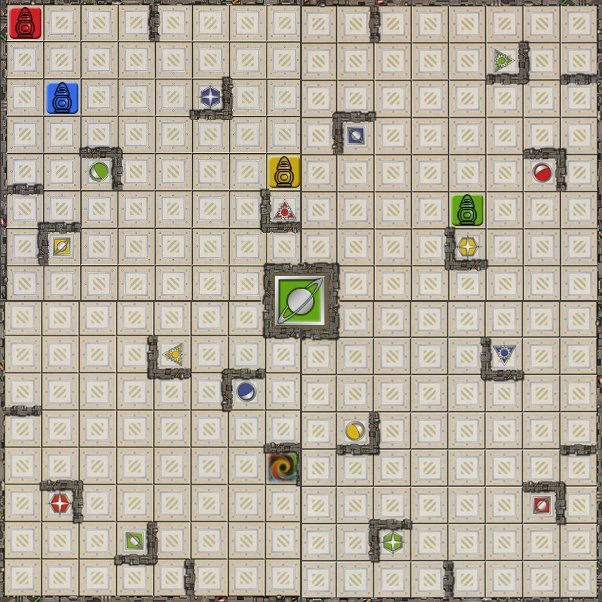
\includegraphics[width=0.7\linewidth]{Thème 1 – Structures de données/Chapitre 1 - Interface et implémentation/BLOB/ricochet-robots-plateau}
\end{center}
Reprenons le même exemple que précédemment. Cette fois vous devez envoyer les instructions avec une file dans un premier temps, puis avec une pile dans un deuxième temps.\\


Exercice 1:
\begin{lstlisting}[language=Python]
    fifo.append("bas")
    fifo.append("bas")
    fifo.append("droite")

    while not fifoq.empty():
        d = fifo.pop(0)
        deplacer_B(d)

\end{lstlisting}
Sur quel repère se trouve le robot bleu?\\

Exercice 2:
\begin{lstlisting}[language=Python]
    fifo.append("haut")
    fifo.append("haut")
    fifo.append("gauche")
    fifo.append("gauche")
    fifo.append("gauche")

    while not fifo.empty():
        d = fifoq.get()
        deplacer_V(d)
\end{lstlisting}
Sur quel repère se trouve le robot vert?\\

Exercice 3:
\begin{lstlisting}[language=Python]
    import queue 

    # Creer une pile LIFO vide 
    fifoq = queue.LifoQueue()

    for i in range(2):
        lifoq.put("bas")
    for i in range(4):
        lifoq.put("droite")
    for i in range(5):
        lifoq.put("bas")
    for i in range(2):
        lifoq.put("gauche")

    while not fifoq.empty():
        d = lifoq.get()
        deplacer_J(d)
\end{lstlisting}
Sur quel repère se trouve le robot jaune?\\

A votre tour de faire jouer les autres !\\




Bravo, vous savez maintenant expliquer les principes théoriques d'une structure de données, en préciser l'interface et implémentation en python les listes, les piles et les files ! 
